\begin{document}
% CVS info. These are modified by cvs at checkout time.
% The last version of these macros found before the maketitle will be the one on the front page,
% so only the main file is tracked.
% Edit by hand with care!
%\RCS$Revision: 1.7 $
%\RCS$Date: 2009/05/12 19:20:52 $
%\RCS$Name:  $
%%%%%%%%%%%%% ptdr definitions %%%%%%%%%%%%%%%%%%%%%
%%%%%%%%%%%%%%%%%%%%%%%%%%%%%%%%%%%%%%%%%%%%%%%%%%%%%%%%%%%%%%%%%%%%
%
%  Common definitions
%
%  N.B. use of \providecommand rather than \newcommand means
%       that a definition is ignored if already specified
%
%                                              L. Taylor 18 Feb 2005
%%%%%%%%%%%%%%%%%%%%%%%%%%%%%%%%%%%%%%%%%%%%%%%%%%%%%%%%%%%%%%%%%%%%

% Some shorthand
% turn off italics
\newcommand {\etal}{\mbox{et al.}\xspace} %et al. - no preceding comma
\newcommand {\ie}{\mbox{i.e.}\xspace}     %i.e.
\newcommand {\eg}{\mbox{e.g.}\xspace}     %e.g.
\newcommand {\etc}{\mbox{etc.}\xspace}     %etc.
\newcommand {\vs}{\mbox{\sl vs.}\xspace}      %vs.
\newcommand {\mdash}{\ensuremath{\mathrm{-}}} % for use within formulas

% some terms whose definition we may change
\newcommand {\Lone}{Level-1\xspace} % Level-1 or L1 ?
\newcommand {\Ltwo}{Level-2\xspace}
\newcommand {\Lthree}{Level-3\xspace}

% Some software programs (alphabetized)
\providecommand{\ACERMC} {\textsc{AcerMC}\xspace}
\providecommand{\ALPGEN} {{\textsc{alpgen}}\xspace}
\providecommand{\CHARYBDIS} {{\textsc{charybdis}}\xspace}
\providecommand{\CMKIN} {\textsc{cmkin}\xspace}
\providecommand{\CMSIM} {{\textsc{cmsim}}\xspace}
\providecommand{\CMSSW} {{\textsc{cmssw}}\xspace}
\providecommand{\COBRA} {{\textsc{cobra}}\xspace}
\providecommand{\COCOA} {{\textsc{cocoa}}\xspace}
\providecommand{\COMPHEP} {\textsc{CompHEP}\xspace}
\providecommand{\EVTGEN} {{\textsc{evtgen}}\xspace}
\providecommand{\FAMOS} {{\textsc{famos}}\xspace}
\providecommand{\GARCON} {\textsc{garcon}\xspace}
\providecommand{\GARFIELD} {{\textsc{garfield}}\xspace}
\providecommand{\GEANE} {{\textsc{geane}}\xspace}
\providecommand{\GEANTfour} {{\textsc{geant4}}\xspace}
\providecommand{\GEANTthree} {{\textsc{geant3}}\xspace}
\providecommand{\GEANT} {{\textsc{geant}}\xspace}
\providecommand{\HDECAY} {\textsc{hdecay}\xspace}
\providecommand{\HERWIG} {{\textsc{herwig}}\xspace}
\providecommand{\HIGLU} {{\textsc{higlu}}\xspace}
\providecommand{\HIJING} {{\textsc{hijing}}\xspace}
\providecommand{\IGUANA} {\textsc{iguana}\xspace}
\providecommand{\ISAJET} {{\textsc{isajet}}\xspace}
\providecommand{\ISAPYTHIA} {{\textsc{isapythia}}\xspace}
\providecommand{\ISASUGRA} {{\textsc{isasugra}}\xspace}
\providecommand{\ISASUSY} {{\textsc{isasusy}}\xspace}
\providecommand{\ISAWIG} {{\textsc{isawig}}\xspace}
\providecommand{\MADGRAPH} {\textsc{MadGraph}\xspace}
\providecommand{\MCATNLO} {\textsc{mc@nlo}\xspace}
\providecommand{\MCFM} {\textsc{mcfm}\xspace}
\providecommand{\MILLEPEDE} {{\textsc{millepede}}\xspace}
\providecommand{\ORCA} {{\textsc{orca}}\xspace}
\providecommand{\OSCAR} {{\textsc{oscar}}\xspace}
\providecommand{\PHOTOS} {\textsc{photos}\xspace}
\providecommand{\PROSPINO} {\textsc{prospino}\xspace}
\providecommand{\PYTHIA} {{\textsc{pythia}}\xspace}
\providecommand{\SHERPA} {{\textsc{sherpa}}\xspace}
\providecommand{\TAUOLA} {\textsc{tauola}\xspace}
\providecommand{\TOPREX} {\textsc{TopReX}\xspace}
\providecommand{\XDAQ} {{\textsc{xdaq}}\xspace}


%  Experiments
\newcommand {\DZERO}{D\O\xspace}     %etc.


% Measurements and units...

\newcommand{\de}{\ensuremath{^\circ}}
\newcommand{\ten}[1]{\ensuremath{\times \text{10}^\text{#1}}}
\newcommand{\unit}[1]{\ensuremath{\text{\,#1}}\xspace}
\newcommand{\mum}{\ensuremath{\,\mu\text{m}}\xspace}
\newcommand{\micron}{\ensuremath{\,\mu\text{m}}\xspace}
\newcommand{\cm}{\ensuremath{\,\text{cm}}\xspace}
\newcommand{\mm}{\ensuremath{\,\text{mm}}\xspace}
\newcommand{\mus}{\ensuremath{\,\mu\text{s}}\xspace}
\newcommand{\keV}{\ensuremath{\,\text{ke\hspace{-.08em}V}}\xspace}
\newcommand{\MeV}{\ensuremath{\,\text{Me\hspace{-.08em}V}}\xspace}
\newcommand{\GeV}{\ensuremath{\,\text{Ge\hspace{-.08em}V}}\xspace}
\newcommand{\TeV}{\ensuremath{\,\text{Te\hspace{-.08em}V}}\xspace}
\newcommand{\PeV}{\ensuremath{\,\text{Pe\hspace{-.08em}V}}\xspace}
\newcommand{\keVc}{\ensuremath{{\,\text{ke\hspace{-.08em}V\hspace{-0.16em}/\hspace{-0.08em}}c}}\xspace}
\newcommand{\MeVc}{\ensuremath{{\,\text{Me\hspace{-.08em}V\hspace{-0.16em}/\hspace{-0.08em}}c}}\xspace}
\newcommand{\GeVc}{\ensuremath{{\,\text{Ge\hspace{-.08em}V\hspace{-0.16em}/\hspace{-0.08em}}c}}\xspace}
\newcommand{\TeVc}{\ensuremath{{\,\text{Te\hspace{-.08em}V\hspace{-0.16em}/\hspace{-0.08em}}c}}\xspace}
\newcommand{\keVcc}{\ensuremath{{\,\text{ke\hspace{-.08em}V\hspace{-0.16em}/\hspace{-0.08em}}c^\text{2}}}\xspace}
\newcommand{\MeVcc}{\ensuremath{{\,\text{Me\hspace{-.08em}V\hspace{-0.16em}/\hspace{-0.08em}}c^\text{2}}}\xspace}
\newcommand{\GeVcc}{\ensuremath{{\,\text{Ge\hspace{-.08em}V\hspace{-0.16em}/\hspace{-0.08em}}c^\text{2}}}\xspace}
\newcommand{\TeVcc}{\ensuremath{{\,\text{Te\hspace{-.08em}V\hspace{-0.16em}/\hspace{-0.08em}}c^\text{2}}}\xspace}

\newcommand{\pbinv} {\mbox{\ensuremath{\,\text{pb}^\text{$-$1}}}\xspace}
\newcommand{\fbinv} {\mbox{\ensuremath{\,\text{fb}^\text{$-$1}}}\xspace}
\newcommand{\nbinv} {\mbox{\ensuremath{\,\text{nb}^\text{$-$1}}}\xspace}
\newcommand{\percms}{\ensuremath{\,\text{cm}^\text{$-$2}\,\text{s}^\text{$-$1}}\xspace}
\newcommand{\lumi}{\ensuremath{\mathcal{L}}\xspace}
\newcommand{\Lumi}{\ensuremath{\mathcal{L}}\xspace}%both upper and lower
%
% Need a convention here:
\newcommand{\LvLow}  {\ensuremath{\mathcal{L}=\text{10}^\text{32}\,\text{cm}^\text{$-$2}\,\text{s}^\text{$-$1}}\xspace}
\newcommand{\LLow}   {\ensuremath{\mathcal{L}=\text{10}^\text{33}\,\text{cm}^\text{$-$2}\,\text{s}^\text{$-$1}}\xspace}
\newcommand{\lowlumi}{\ensuremath{\mathcal{L}=\text{2}\times \text{10}^\text{33}\,\text{cm}^\text{$-$2}\,\text{s}^\text{$-$1}}\xspace}
\newcommand{\LMed}   {\ensuremath{\mathcal{L}=\text{2}\times \text{10}^\text{33}\,\text{cm}^\text{$-$2}\,\text{s}^\text{$-$1}}\xspace}
\newcommand{\LHigh}  {\ensuremath{\mathcal{L}=\text{10}^\text{34}\,\text{cm}^\text{$-$2}\,\text{s}^\text{$-$1}}\xspace}
\newcommand{\hilumi} {\ensuremath{\mathcal{L}=\text{10}^\text{34}\,\text{cm}^\text{$-$2}\,\text{s}^\text{$-$1}}\xspace}

% Some usual physics terms


% SM (still to be classified)

\newcommand{\kt}{\ensuremath{k_{\mathrm{T}}}\xspace}
\newcommand{\BC}{\ensuremath{{B_{\mathrm{c}}}}\xspace}
\newcommand{\bbarc}{\ensuremath{{\overline{b}c}}\xspace}
\newcommand{\bbbar}{\ensuremath{{b\overline{b}}}\xspace}
\newcommand{\ccbar}{\ensuremath{{c\overline{c}}}\xspace}
\newcommand{\JPsi}{\ensuremath{{J}\hspace{-.08em}/\hspace{-.14em}\psi}\xspace}
\newcommand{\bspsiphi}{\ensuremath{B_s \to \JPsi\, \phi}\xspace}
%\newcommand{\ttbar}{\ensuremath{{t\overline{t}}}\xspace}
\newcommand{\AFB}{\ensuremath{A_\text{FB}}\xspace}
\newcommand{\EE}{\ensuremath{e^+e^-}\xspace}
\newcommand{\MM}{\ensuremath{\mu^+\mu^-}\xspace}
\newcommand{\TT}{\ensuremath{\tau^+\tau^-}\xspace}
\newcommand{\wangle}{\ensuremath{\sin^{2}\theta_{\text{eff}}^\text{lept}(M^2_\mathrm{Z})}\xspace}
\newcommand{\ttbar}{\ensuremath{{t\overline{t}}}\xspace}
\newcommand{\stat}{\ensuremath{\,\text{(stat.)}}\xspace}
\newcommand{\syst}{\ensuremath{\,\text{(syst.)}}\xspace}
% these moved to similar defs
%\newcommand{\Etmiss}{\ensuremath{E_{\mathrm{T}\!{\rm miss}}}}
%\newcommand{\VEtmiss}{\ensuremath{{\vec E}_{\mathrm{T}\!{\rm miss}}}}

%%%  E-gamma definitions
\newcommand{\HGG}{\ensuremath{\mathrm{H}\to\gamma\gamma}}
\newcommand{\gev}{\GeV}
\newcommand{\GAMJET}{\ensuremath{\gamma + \text{jet}}}
\newcommand{\PPTOJETS}{\ensuremath{\mathrm{pp}\to\text{jets}}}
\newcommand{\PPTOGG}{\ensuremath{\mathrm{pp}\to\gamma\gamma}}
\newcommand{\PPTOGAMJET}{\ensuremath{\mathrm{pp}\to\gamma +
\mathrm{jet}
}}
\newcommand{\MH}{\ensuremath{\mathrm{M_{\mathrm{H}}}}}
\newcommand{\RNINE}{\ensuremath{\mathrm{R}_\mathrm{9}}}
\newcommand{\DR}{\ensuremath{\Delta\mathrm{R}}}



% Physics symbols ...

\newcommand{\PT}{\ensuremath{p_{\mathrm{T}}}\xspace}
\newcommand{\pt}{\ensuremath{p_{\mathrm{T}}}\xspace}
\newcommand{\ET}{\ensuremath{E_{\mathrm{T}}}\xspace}
\newcommand{\HT}{\ensuremath{H_{\mathrm{T}}}\xspace}
\newcommand{\et}{\ensuremath{E_{\mathrm{T}}}\xspace}
\providecommand{\Em}{\ensuremath{E\hspace{-0.6em}/}\xspace}
\providecommand{\Pm}{\ensuremath{p\hspace{-0.5em}/}\xspace}
\providecommand{\PTm}{\ensuremath{{p}_\mathrm{T}\hspace{-1.02em}/}\xspace}
\providecommand{\PTslash}{\ensuremath{{p}_\mathrm{T}\hspace{-1.02em}/}\xspace}
\newcommand{\ETm}{\ensuremath{E_{\mathrm{T}}^{\text{miss}}}\xspace}
\providecommand{\ETslash}{\ensuremath{E_{\mathrm{T}}\hspace{-1.1em}/}\xspace}
\newcommand{\MET}{\ensuremath{E_{\mathrm{T}}^{\text{miss}}}\xspace}
\newcommand{\ETmiss}{\ensuremath{E_{\mathrm{T}}^{\text{miss}}}\xspace}
\newcommand{\VEtmiss}{\ensuremath{{\vec E}_{\mathrm{T}}^{\text{miss}}}\xspace}

% roman face derivative
\providecommand{\dd}[2]{\ensuremath{\frac{\mathrm{d} #1}{\mathrm{d} #2}}}
% Particle names which will track the italic/non-italic face convention
\providecommand{\zp}{\ensuremath{\mathrm{Z}^\prime}\xspace}
\providecommand{\JPsi}{\ensuremath{\mathrm{J}\hspace{-.08em}/\hspace{-.14em}\psi}\xspace}
\providecommand{\Z}{\ensuremath{\mathrm{Z}}\xspace}
\providecommand{\ttbar}{\ensuremath{\mathrm{t}\overline{\mathrm{t}}}\xspace}
% Extensions for missing names in PENNAMES
\providecommand{\cPgn}{\ensuremath{\nu}\xspace} % generic neutrino
\providecommand{\cPJgy}{\JPsi} % J/Psi (no mass)
\providecommand{\cPZ}{\Z} % plain Z (no superscript 0)
\providecommand{\cPZpr}{\zp} % plain Z'
% SymbolFace not yet available in trunk version
%\providecommand{\cPqb}{\ensuremath{\cmsSymbolFace{b}}\xspace} % b for b quark
%\providecommand{\cPqt}{\ensuremath{\cmsSymbolFace{t}}\xspace} % t for t quark
%\providecommand{\cPqc}{\ensuremath{\cmsSymbolFace{c}}\xspace} % c for c quark
%\providecommand{\cPaqb}{\ensuremath{\overline{\cmsSymbolFace{b}}\xspace}} % b for b anti-quark
%\providecommand{\cPaqt}{\ensuremath{\overline{\cmsSymbolFace{t}}}\xspace} % t for t anti-quark
%\providecommand{\cPaqc}{\ensuremath{\overline{\cmsSymbolFace{c}}}\xspace} % c for c anti-quark
%%%%%%
% From Albert
%

\newcommand{\ga}{\ensuremath{\gtrsim}}
\newcommand{\la}{\ensuremath{\lesssim}}
%\def\ga{\mathrel{\rlap{\raise.6ex\hbox{$>$}}{\lower.6ex\hbox{$\sim$}}}}
%\def\la{\mathrel{\rlap{\raise.6ex\hbox{$<$}}{\lower.6ex\hbox{$\sim$}}}}
%
\newcommand{\swsq}{\ensuremath{\sin^2\theta_W}\xspace}
\newcommand{\cwsq}{\ensuremath{\cos^2\theta_W}\xspace}
\newcommand{\tanb}{\ensuremath{\tan\beta}\xspace}
\newcommand{\tanbsq}{\ensuremath{\tan^{2}\beta}\xspace}
\newcommand{\sidb}{\ensuremath{\sin 2\beta}\xspace}
\newcommand{\alpS}{\ensuremath{\alpha_S}\xspace}
\newcommand{\alpt}{\ensuremath{\tilde{\alpha}}\xspace}

\newcommand{\QL}{\ensuremath{Q_L}\xspace}
\newcommand{\sQ}{\ensuremath{\tilde{Q}}\xspace}
\newcommand{\sQL}{\ensuremath{\tilde{Q}_L}\xspace}
\newcommand{\ULC}{\ensuremath{U_L^C}\xspace}
\newcommand{\sUC}{\ensuremath{\tilde{U}^C}\xspace}
\newcommand{\sULC}{\ensuremath{\tilde{U}_L^C}\xspace}
\newcommand{\DLC}{\ensuremath{D_L^C}\xspace}
\newcommand{\sDC}{\ensuremath{\tilde{D}^C}\xspace}
\newcommand{\sDLC}{\ensuremath{\tilde{D}_L^C}\xspace}
\newcommand{\LL}{\ensuremath{L_L}\xspace}
\newcommand{\sL}{\ensuremath{\tilde{L}}\xspace}
\newcommand{\sLL}{\ensuremath{\tilde{L}_L}\xspace}
\newcommand{\ELC}{\ensuremath{E_L^C}\xspace}
\newcommand{\sEC}{\ensuremath{\tilde{E}^C}\xspace}
\newcommand{\sELC}{\ensuremath{\tilde{E}_L^C}\xspace}
\newcommand{\sEL}{\ensuremath{\tilde{E}_L}\xspace}
\newcommand{\sER}{\ensuremath{\tilde{E}_R}\xspace}
\newcommand{\sFer}{\ensuremath{\tilde{f}}\xspace}
\newcommand{\sQua}{\ensuremath{\tilde{q}}\xspace}
\newcommand{\sUp}{\ensuremath{\tilde{u}}\xspace}
\newcommand{\suL}{\ensuremath{\tilde{u}_L}\xspace}
\newcommand{\suR}{\ensuremath{\tilde{u}_R}\xspace}
\newcommand{\sDw}{\ensuremath{\tilde{d}}\xspace}
\newcommand{\sdL}{\ensuremath{\tilde{d}_L}\xspace}
\newcommand{\sdR}{\ensuremath{\tilde{d}_R}\xspace}
\newcommand{\sTop}{\ensuremath{\tilde{t}}\xspace}
\newcommand{\stL}{\ensuremath{\tilde{t}_L}\xspace}
\newcommand{\stR}{\ensuremath{\tilde{t}_R}\xspace}
\newcommand{\stone}{\ensuremath{\tilde{t}_1}\xspace}
\newcommand{\sttwo}{\ensuremath{\tilde{t}_2}\xspace}
\newcommand{\sBot}{\ensuremath{\tilde{b}}\xspace}
\newcommand{\sbL}{\ensuremath{\tilde{b}_L}\xspace}
\newcommand{\sbR}{\ensuremath{\tilde{b}_R}\xspace}
\newcommand{\sbone}{\ensuremath{\tilde{b}_1}\xspace}
\newcommand{\sbtwo}{\ensuremath{\tilde{b}_2}\xspace}
\newcommand{\sLep}{\ensuremath{\tilde{l}}\xspace}
\newcommand{\sLepC}{\ensuremath{\tilde{l}^C}\xspace}
\newcommand{\sEl}{\ensuremath{\tilde{e}}\xspace}
\newcommand{\sElC}{\ensuremath{\tilde{e}^C}\xspace}
\newcommand{\seL}{\ensuremath{\tilde{e}_L}\xspace}
\newcommand{\seR}{\ensuremath{\tilde{e}_R}\xspace}
\newcommand{\snL}{\ensuremath{\tilde{\nu}_L}\xspace}
\newcommand{\sMu}{\ensuremath{\tilde{\mu}}\xspace}
\newcommand{\sNu}{\ensuremath{\tilde{\nu}}\xspace}
\newcommand{\sTau}{\ensuremath{\tilde{\tau}}\xspace}
\newcommand{\Glu}{\ensuremath{g}\xspace}
\newcommand{\sGlu}{\ensuremath{\tilde{g}}\xspace}
\newcommand{\Wpm}{\ensuremath{W^{\pm}}\xspace}
\newcommand{\sWpm}{\ensuremath{\tilde{W}^{\pm}}\xspace}
\newcommand{\Wz}{\ensuremath{W^{0}}\xspace}
\newcommand{\sWz}{\ensuremath{\tilde{W}^{0}}\xspace}
\newcommand{\sWino}{\ensuremath{\tilde{W}}\xspace}
\newcommand{\Bz}{\ensuremath{B^{0}}\xspace}
\newcommand{\sBz}{\ensuremath{\tilde{B}^{0}}\xspace}
\newcommand{\sBino}{\ensuremath{\tilde{B}}\xspace}
\newcommand{\Zz}{\ensuremath{Z^{0}}\xspace}
\newcommand{\sZino}{\ensuremath{\tilde{Z}^{0}}\xspace}
\newcommand{\sGam}{\ensuremath{\tilde{\gamma}}\xspace}
\newcommand{\chiz}{\ensuremath{\tilde{\chi}^{0}}\xspace}
\newcommand{\chip}{\ensuremath{\tilde{\chi}^{+}}\xspace}
\newcommand{\chim}{\ensuremath{\tilde{\chi}^{-}}\xspace}
\newcommand{\chipm}{\ensuremath{\tilde{\chi}^{\pm}}\xspace}
\newcommand{\Hone}{\ensuremath{H_{d}}\xspace}
\newcommand{\sHone}{\ensuremath{\tilde{H}_{d}}\xspace}
\newcommand{\Htwo}{\ensuremath{H_{u}}\xspace}
\newcommand{\sHtwo}{\ensuremath{\tilde{H}_{u}}\xspace}
\newcommand{\sHig}{\ensuremath{\tilde{H}}\xspace}
\newcommand{\sHa}{\ensuremath{\tilde{H}_{a}}\xspace}
\newcommand{\sHb}{\ensuremath{\tilde{H}_{b}}\xspace}
\newcommand{\sHpm}{\ensuremath{\tilde{H}^{\pm}}\xspace}
\newcommand{\hz}{\ensuremath{h^{0}}\xspace}
\newcommand{\Hz}{\ensuremath{H^{0}}\xspace}
\newcommand{\Az}{\ensuremath{A^{0}}\xspace}
\newcommand{\Hpm}{\ensuremath{H^{\pm}}\xspace}
\newcommand{\sGra}{\ensuremath{\tilde{G}}\xspace}
%
\newcommand{\mtil}{\ensuremath{\tilde{m}}\xspace}
%
\newcommand{\rpv}{\ensuremath{\rlap{\kern.2em/}R}\xspace}
\newcommand{\LLE}{\ensuremath{LL\bar{E}}\xspace}
\newcommand{\LQD}{\ensuremath{LQ\bar{D}}\xspace}
\newcommand{\UDD}{\ensuremath{\overline{UDD}}\xspace}
\newcommand{\Lam}{\ensuremath{\lambda}\xspace}
\newcommand{\Lamp}{\ensuremath{\lambda'}\xspace}
\newcommand{\Lampp}{\ensuremath{\lambda''}\xspace}
%
\newcommand{\spinbd}[2]{\ensuremath{\bar{#1}_{\dot{#2}}}\xspace}

\newcommand{\MD}{\ensuremath{{M_\mathrm{D}}}\xspace}% ED mass
\newcommand{\Mpl}{\ensuremath{{M_\mathrm{Pl}}}\xspace}% Planck mass
\newcommand{\Rinv} {\ensuremath{{R}^{-1}}\xspace}



%%%%%%%%%%%%%%%%%%%%%%%%%%%%%%%%%%%%%%%%%%%%%%%%%%%%%%%%%%%%%%%%%%%%
%
% Hyphenations (only need to add here if you get a nasty word break)
%
\hyphenation{en-viron-men-tal}%    just an example

%%%%%%%%%%%%%%%  Title page %%%%%%%%%%%%%%%%%%%%%%%%
% [Not required for PAS notes -- derived from directory name.] Please replace 2006/000 with your note number in the following line:
%\cmsNoteHeader{XXX-08-000}
\title{EJ200 Scintillator Tile Geometry Update and Testing}% Force line breaks with \\

%\address[cern]{CERN}
%\address[neu]{Northeastern University}
%\author[neu]{George Alverson}
%\author[neu]{Lucas Taylor}
%\author[cern]{A. Cern Person}
\author{A. Horst}

% please supply the date in yyyy/mm/dd format. Today has been
% redefined to do so, but it should be fixed as of the final release date.
\date{\today}

% note that you cannot use \verb in the abstract text
\abstract{
We study the light output and light collection efficiency of the EJ-200 Scintillator Tile by Eljen Technology, using a simulated tile created using GEANT4 software. We present new methods of testing uniformity and efficiency of irradiated and unirradiated simulated tiles.

}

% these need to be filled in by hand and should (MUST) match the info
% in the TeX equivalents less the TeX markup
\hypersetup{%
pdfauthor={A. Horst},%
pdftitle={EJ-200 Scintillator Tile Geometry Update and Testing in GEANT4},%
pdfsubject={CMS},%
pdfkeywords={CMS, physics, software, computing}}
\maketitle %maketitle comes after all the front information has been supplied

%%%%%%%%%%%%%%%%%%%%%%%%%%%%%%%%  Begin text %%%%%%%%%%%%%%%%%%%%%%%%%%%%%

\section{CMS papers}
We study the light output and collection efficiency of scintillators being considered for an update at the hadronic calorimeter of the CMS detector. Experimental tests are useful for determining properties of different tiles, however, simulations using GEANT4 could provide another more efficient way of testing different geometries and tiles. Here I test a commercial scintillator by Eljen Technology: the EJ-200 tile. It has a polyvinyltoluene (PVT) base, an emission peak of 425nm, a σ shaped groove with a wavelength shifting fiber inside connected to a Hamamatsu R6091 PMT and is wrapped in Tyvek.

\begin{figure}[h!]
  \begin{center}
    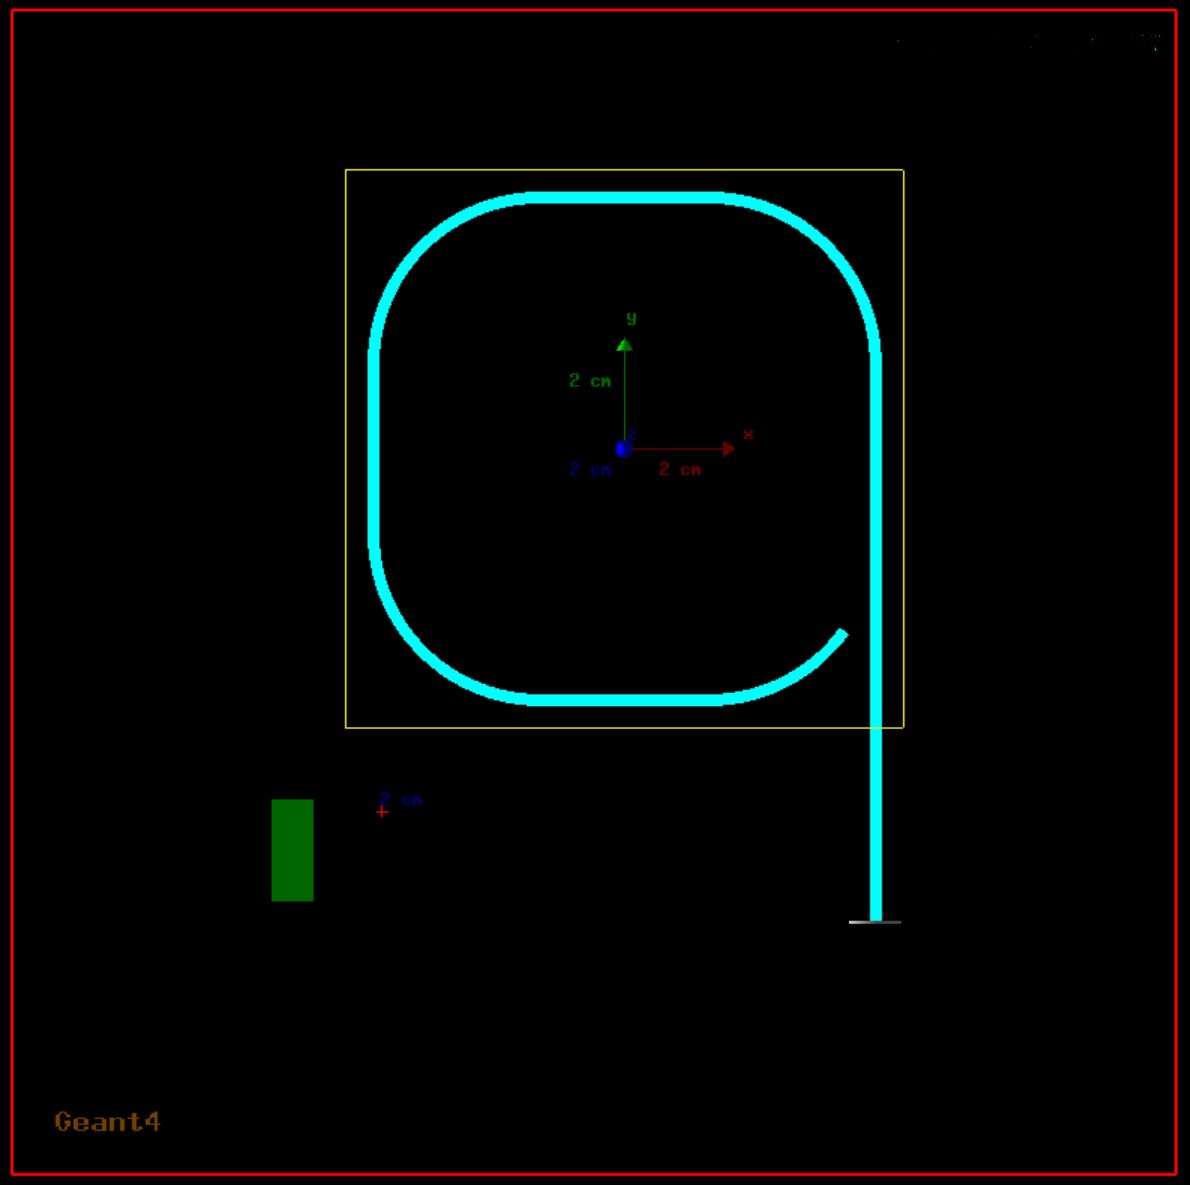
\includegraphics[width=0.42\textwidth]{Curved.JPG}
    \caption{Visual simulation of the new fiber (blue) for the EJ-200 simulated tile.}
    \label{fig:1}
  \end{center}
\end{figure}

\section{Project}
	Our tile simulation was in need of a modified geometry for the EJ-200 material. The main section altered was the output corner, where the fiber leaves the tile, and where the opposite end of the fiber ends inside the tile. Originally, the output of the fiber was connected to the end of the fiber in a T like style on the output corner. This is not true of the EJ-200 tile, in which the end and output are not connected at this corner, nor is the end of the fiber straight. The EJ-200 fiber looks closer to a σ, where the output is not connected to the end of the Fiber (see Fig.~\ref{fig:1}). 

\begin{figure}[h!]
  \begin{center}
    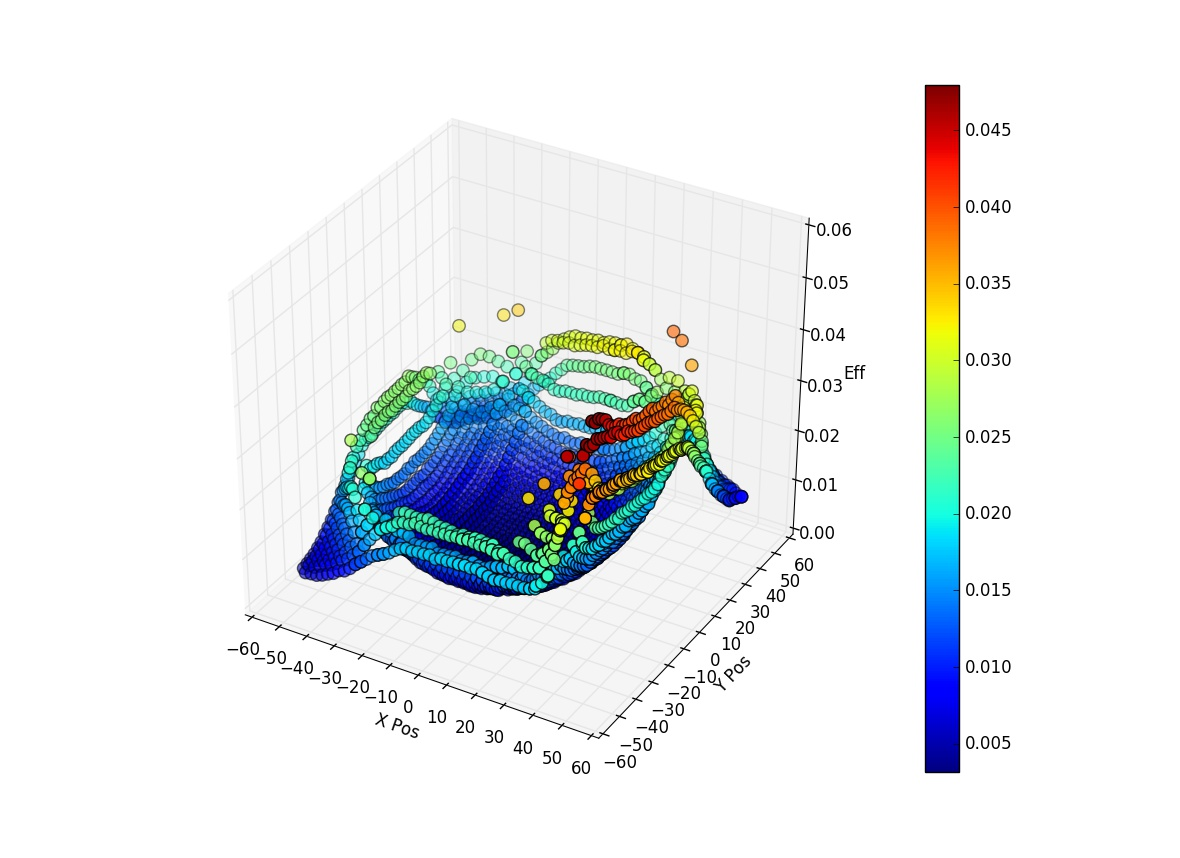
\includegraphics[width=0.6\textwidth]{figure_2.jpeg}
    \caption{Example of a 2500 point efficiency simulation with 1 million events per point at 1 photon per event, on the unirradiated tile simulation (with points inside the fiber removed due to their outlying nature). Efficiencies are very low, as expected. Even with thousands of emitted photons, only a few are likely to be recorded.}
    \label{fig:2}
  \end{center}
\end{figure}

\subsection{Uniformity Testing}
	To test this new geometry, and create ways of validating new tile geometries with the GEANT4 simulation, I added a method to test uniformity of photon detection efficiency in the tile. Other experimental researchers provided absorption lengths from tests with irradiated and unirradiated tiles. Using these experimental results, I was able to find the uniformity of photon absorption in the simulated tile based on position. This involved creating a function to record the photon source position to gather position based data on the number of photons being detected by the unirradiated and irradiated tiles. Although partially used to compare the unirradiated tiles to the irradiated tiles, this process was also used to observe the accuracy of the simulation itself, by comparing the results to known, measured results. To complete this uniformity test, I needed a method of creating a changing particle source to test specific points on the tile. Using the position commands and a python script, I could run multiple jobs at different points. I also added a function that records the position of the particle source before each run, so my final results could be differentiated by their source position. Fig.~\ref{fig:2} shows an example of the results from this testing, with a position based graph of the efficiency of the tile at picking up photons from a photon source with 2500 points total each with 1 million events of 1 photon randomly shot from the center plane of the tile in any direction. Fig.~\ref{fig:3} displays the ratio of an irradiated tile to an unirradiated tile’s efficiency.

\begin{figure}[h!]
  \begin{center}
    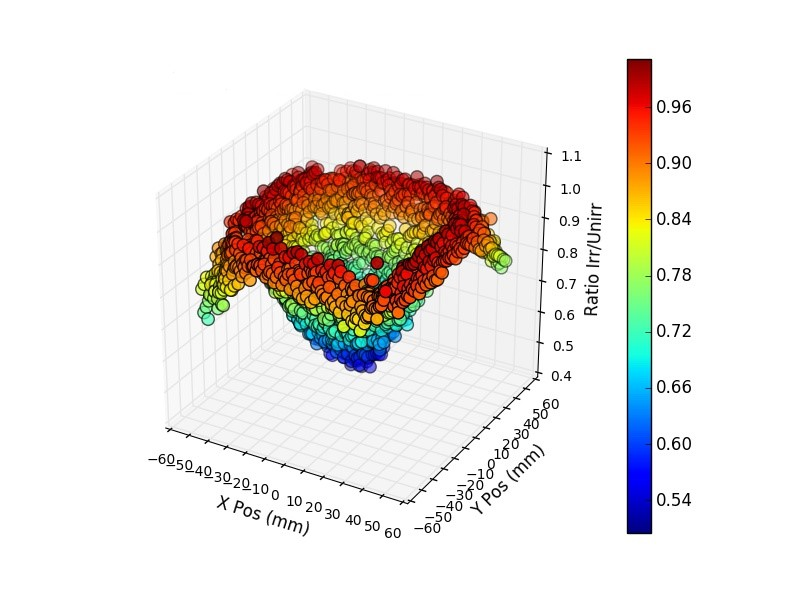
\includegraphics[width=0.6\textwidth]{figure_2-1.jpeg}
    \caption{Ratio between the efficiencies (photons that reach the PMT vs photons released from the particle source) of the irradiated vs the unirradiated tiles at 2500 points. Results show similar efficiencies around the fiber groove and ratios as low as .5 in the center of the tile, where the light travels through more of the scintillator, and is more likely to be absorbed in the irradiated tile before reaching the fiber.}
    \label{fig:3}
  \end{center}
\end{figure}

\subsection{Muon Light Yield Testing}
	In addition to tile uniformity testing, I needed a way to find an estimated number of photons released in the EJ-200 tile by Muons interacting with it, causing scintillation. This was done in part by observing the number of detected photons in a simulation given a certain number of photons released from a particle source. I also used histograms to record the amount of energy deposited in the simulated scintillator by a Muon of energy given by a sea level muon distribution \cite{hlw07}. This could be used to narrow down the number of photons that might be released during scintillation of Muons in the EJ-200 tile.

\begin{figure}[h!]
  \begin{center}
    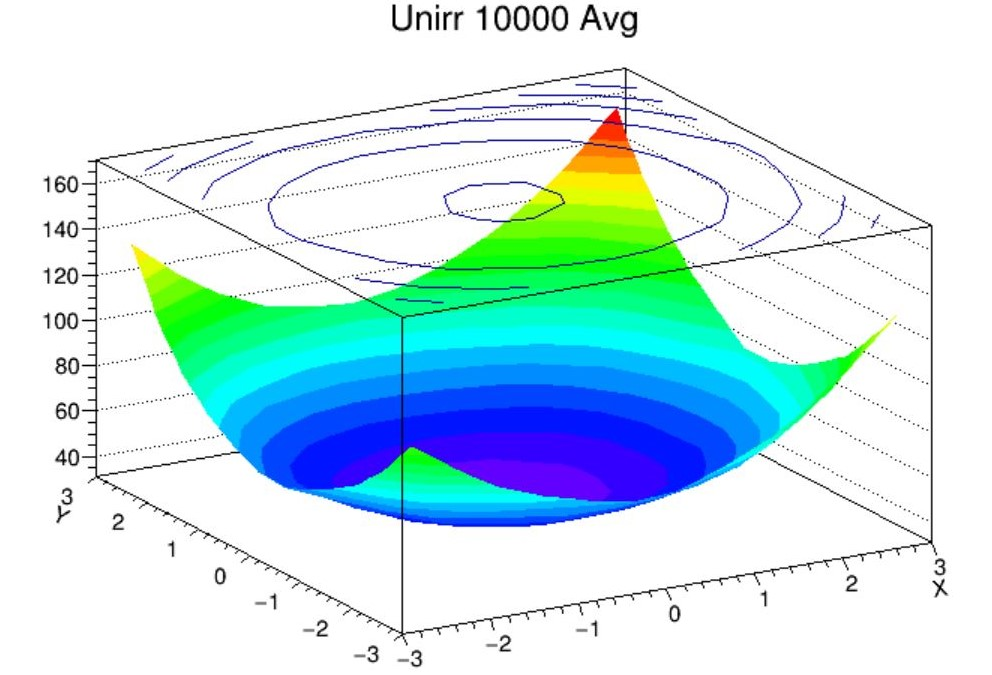
\includegraphics[width=0.4\textwidth]{Unirr10000Avg.JPG}
    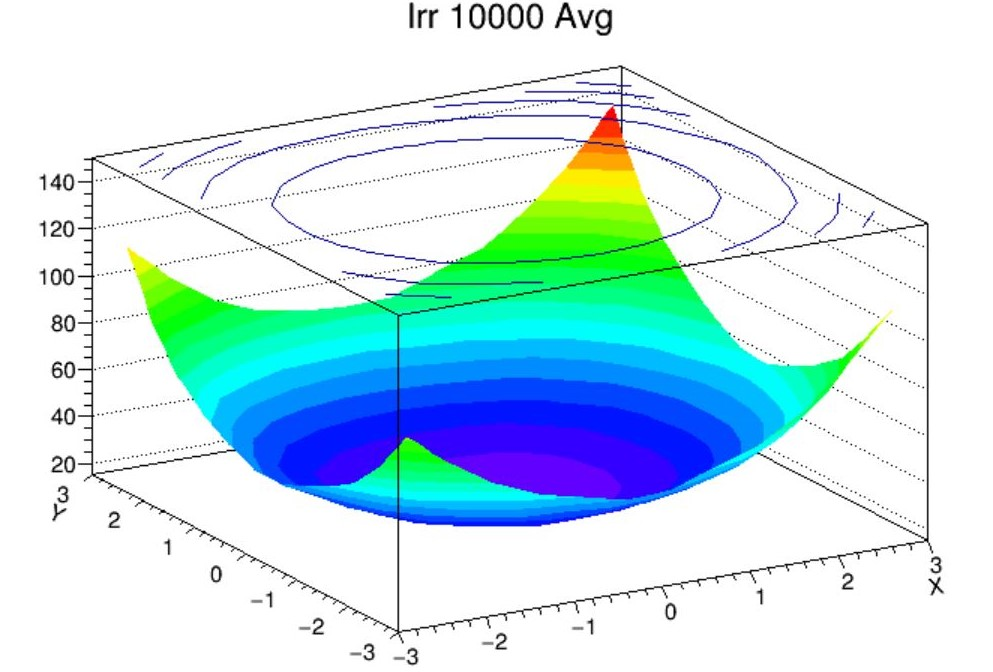
\includegraphics[width=0.4\textwidth]{Irr10000Avg.JPG}
    \caption{Avg number of photons detected out of 1000 events with 10000 photons at 400 points on the irradiated and unirradiated tiles (graphed in the center of the tile in area enclosed by fiber).}
    \label{fig:4}
  \end{center}
\end{figure}

\section{Function}
e primary goal of this project is to modify/extend and verify our existing GEANT4 simulation, including updating the tile geometry of the scintillator tile to the commercial EJ-200 geometry, by altering the tile geometry and the fiber groove. This change was made so I could more realistically describe real measurements, such as the cosmic ray, alpha source, and test beam measurements, which could then be used to explain behaviors in the real tiles. After validating these results, others can further develop this simulation based on this simulation to morph/extrapolate it into more geometries for other tiles. By comparing/contrasting different types/geometries of tiles, one could find tiles better suited for use in the detector based on radiation damage, longevity, and accuracy. These tiles are crucial to the measurements made at CMS, and better tiles will mean more accurate measurement with reduced noise. Using GEANT4 will be a straight forward method of finding tiles that best suit the detectors. 

\begin{figure}[h!]
  \begin{center}
    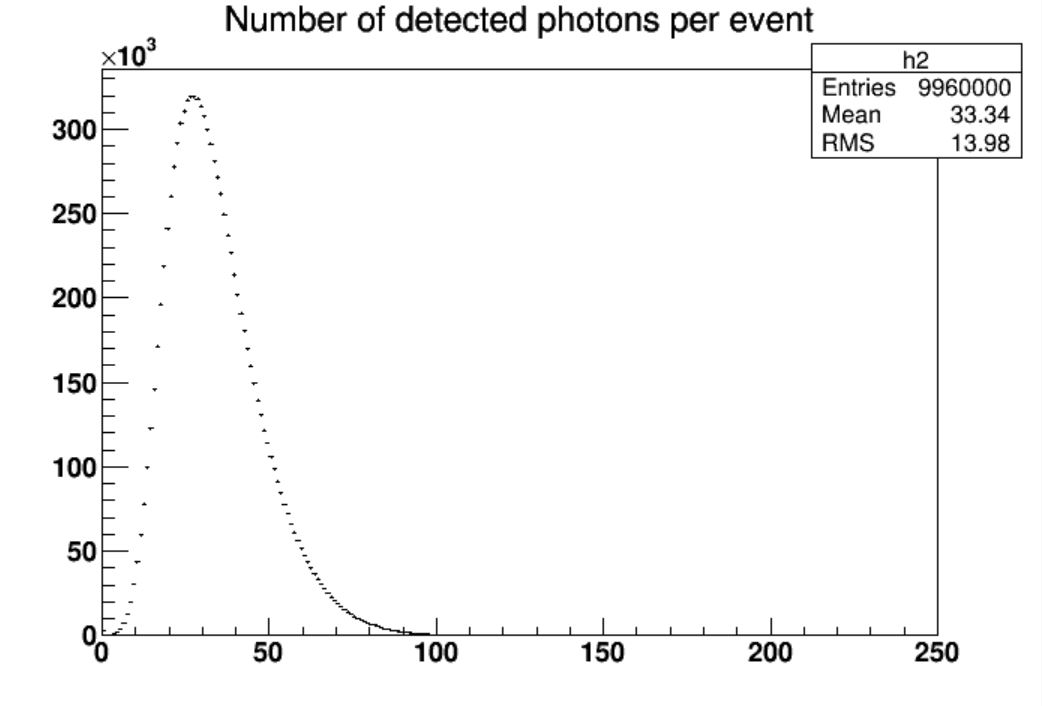
\includegraphics[width=0.4\textwidth]{5000PhotonUnirr(0,250).JPG}\hspace{1cm}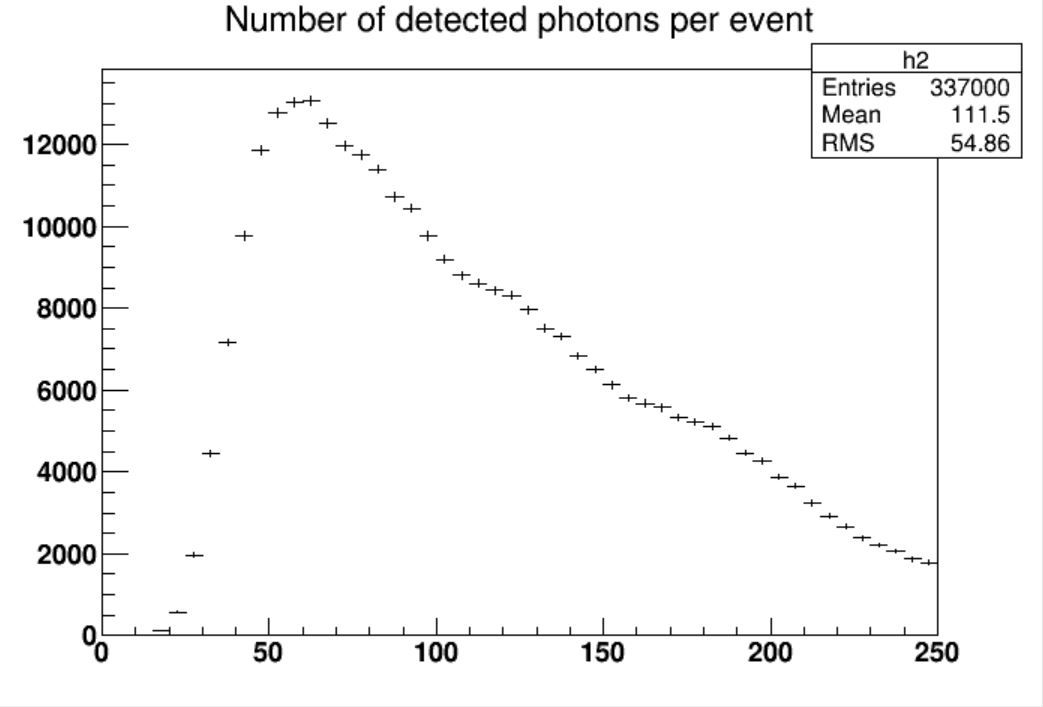
\includegraphics[width=0.4\textwidth]{Fixed10000Unirr.JPG}
    \hspace{1cm}
    \caption{Fig 5. - 5000 photon source histogram of photons detected in ~10 million events with randomly distributed particle source positions along a 9x9cm square plane centered in the middle of the tile.  Fig 6 - 10,000 photon source histogram of photons detected in ~300,000 events, from same source as fig. 5.}
    \label{fig:5,6}
  \end{center}
\end{figure}


\section{Method}
	To test the tiles, I first updated the fiber geometry, which required mostly some slight changes to the tori/tubes that represent the fiber in the simulation. Using previously defined lengths and parameters, I added a new fiber geometry that altered the readout corner to incorporate the new geometry specified earlier. 
\begin{verbatim}
	G4VSolid* solidFiberCurved1R = 
        new G4Torus(name+"CurvedSection1R",
                    radiusI,                        //G4double pRmin,
                    radiusO,                        //G4double pRmax,
                    bendRadius,                     //G4double pRtor,
                    1.5*pi,       	            //G4double pSPhi,
                    0.3*pi);      	            //G4double pDPhi)
\end{verbatim}
This code defines a torus for the readout corner, you should notice that the torus does not complete an entire 0.5pi curve (0.3pi in this case), which is what we desire here. Highlighting the fiber in a visual simulation was extremely useful for determining problems.
	The next step was to create a function to record the position of the particle source at the beginning of each event. This was necessary for obtaining the results for each event at each position.
\begin{verbatim}
const G4ThreeVector LYSimPrimaryGeneratorAction::GetSourcePosition()
{
    G4ThreeVector pos = particleSource->GetParticlePosition();
    return pos;
}
\end{verbatim}
To get the output, I recalled \verb|pos| at the end of each run, and I could then associate efficiencies with their original particle source position. I could then make these results into a dataframe using python, and represent the results in a 3d scatter graph using matplotlib. Each simulation I ran had an accompanying python script to submit each simulation job. This script would change certain parameters (source position, histogram names, etc.) and would also submit only the desired jobs, which was important when some points contained unusable points. Additionally, I had the script skip over source positions that were inside the fiber, since they were extraneous and would skew data. 
	Histograms are easily defined in the analysis code, with binning and axis limits (changeable to some degree with root). Filling the histograms is made easy by the singleton access method \verb|Instance()| in the G4AnalysisManager class, meaning histograms can be filled just about anywhere. This was useful when working with muons, since some histograms had to be filled every step, to record the energy deposited into the tile. 


\section{Results}
	The uniformity tests had good results, with some variation of ~4\% (in efficiency) from maximum to minimum, which varied according to the source distance from the fiber and the source distance from the readout corner. At these points, photons incident on the fiber are likely to be detected, of which there are many at these source points in comparison. With a median eff on the unirradiated tile of .012, and a min and max of, respectively .003 and .048 the majority of points lie below 2\% efficiency. This indicates some uniformity in the areas of the tile further from the fiber. The fiber proximity issue also arises when comparing the unirradiated and irradiated tiles, as depicted in Fig.~\ref{fig:3}, where the ratios in these areas are close to 1, whereas in central/corner areas the ratios drop below 1 (as expected). These results demonstrate the capabilities of the tile simulation to test scintillator tiles for use in detectors. These tests show methods of comparing tiles in terms of uniformity, and degradation. This may prove to be an important method in testing new styles of tile geometries.
	The muon tests were ultimately to get a bound on the number of photons detected compared to the amount released at the particle source.  Both have a positive skew gaussian distribution which gets more skewed as the source photon count increases. The skewness is likely simply caused by the bound at 0 photons. It is unlikely that 0 photons are recorded in either of these cases, so the distribution has a cut off. The left side of the distribution would be less likely to move outwards (low photon count is still possible and likely) but the right side (higher photon count) expands outwards (possible but less likely). The highest percent of photons absorbed vs. released grow also, the 5,000 photon source curve ends at around 1.5\% (75 photons), the 10,000 photon distribution ends at around 3\% (300).  These results demonstrate how the simulation can be used to find an approximate bound on the number of photons being scintillated when a muon passes through the tile. 


\bibliography{auto_generated}   % will be created by the tdr script.
\clearpage
\appendix